\documentclass[a4paper]{scrartcl}

\usepackage{amsmath}
\usepackage{amsfonts}
\usepackage{amssymb}

\usepackage{amsthm}
\usepackage{stmaryrd}
\usepackage[all]{xy}
\usepackage{color}
\definecolor{darkblue}{rgb}{0,0,.5}
%\usepackage[pdftex, plainpages = false, pdfpagelabels, colorlinks=true,
%breaklinks=true, linkcolor=darkblue, menucolor=darkblue, pagecolor=darkblue, urlcolor=darkblue, citecolor=darkblue, anchorcolor=darkblue 
%]{hyperref}
\usepackage{graphicx,color}
\usepackage{framed}
\usepackage{listings}

%typography extras :-)
\usepackage{microtype}
%\usepackage{ellipsis}

\title{Computational Geometry -- Exercise 6}
\author{Robert K\"unnemann (2512815)}

\begin{document}

\maketitle

\section*{Bounding Box}

Every line can be expressed by a slope and its intersection point with the y-axis, so let the i-th line $L_i$ be defined by
$$ y = a_1x + b_1$$
Our first goal now is to find the left most intersection between two such lines. Based on this, computing the bounding box will be easy. Consider a vertical line $L$ that lies very, very far to the left of the arrangement. Imagine how the other Lines $L_1 \dots L_n$ intersect this line: we see that the slope is material to the order in which they do it (see Fig.~\ref{fig:task1}. If $a_i > a_j$ there is an $y$ from which on for every vertical line through $y'<y$, $L_i$ would intersect it \emph{above} the intersection with $L_j$. If two lines are parallel, of course the $b$-value is important. Therefore we order the lines lexicographically by $(a_i, b_i)$ and hence know in which order they would intersect this imaginary line. Now, if there are two lines that are not adjacent to each other in this ordering, they may very well have an intersection, but: an intersection of one of those lines with another line in between them will have an intersection that is closer to $L$ (or maybe exactly hits their intersection). Therefore our algorithm only has consider every pair of adjacent lines as candidate intersections, which works in $O(n)$. The leftmost intersection if obviously the intersection with minimal x-coordinate. It is because of the sorting set that we have $O(n~log~n)$. 

In order to find the right-most intersection, we imagine $L$ to be on the right-hand side, so we would reverse the order, but the neighbours stay the same anyway. Just that know we search for the maximum $y$ value. Searching for the top and bottom intersection works the same, we would just exchange x and y coordinates for the sake of computation. So we basically do the sorting twice, so the overall running time is $O(n~log~n)$.
\begin{figure}[h]
  \begin{center}
    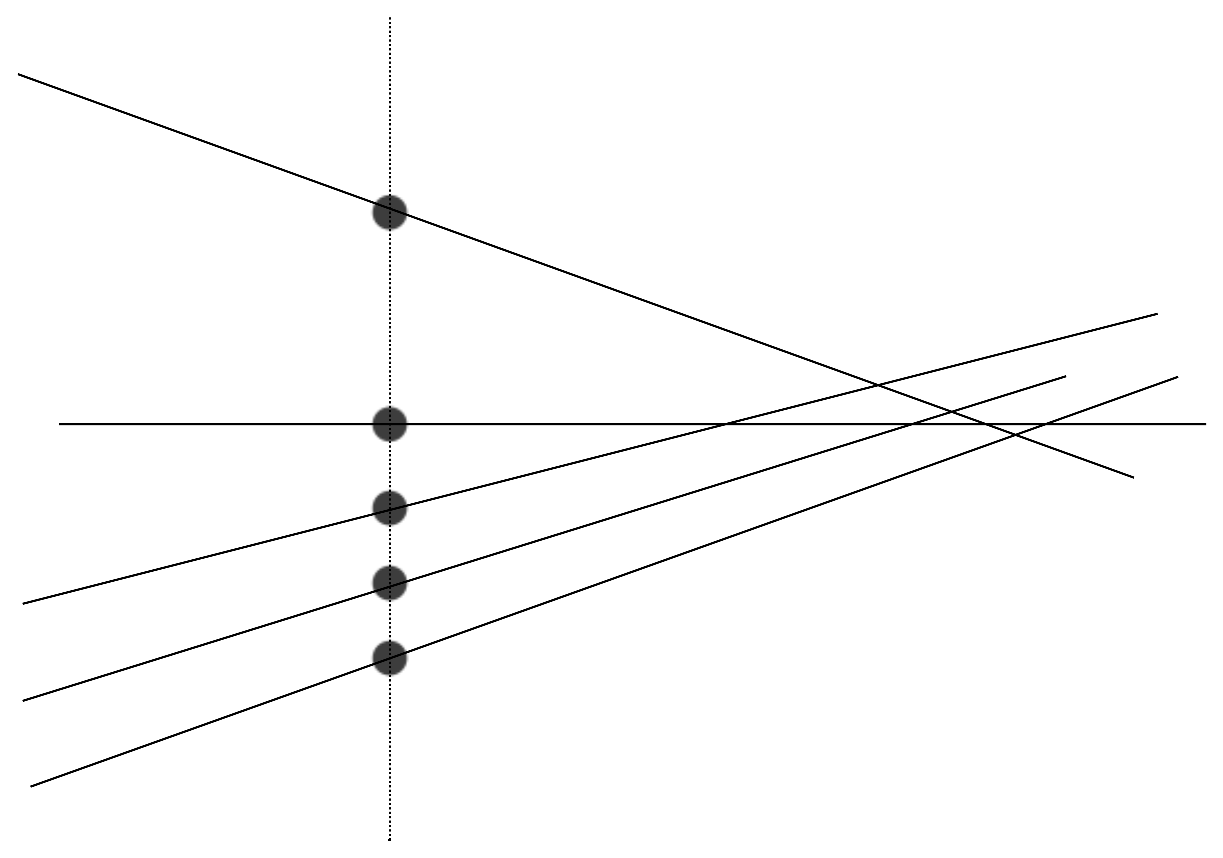
\includegraphics[height=5cm]{pic/task1.eps}
  \end{center}
  \caption{The Line L intersects a lot of lines.}
  \label{fig:task1}
\end{figure}


\section*{Zone of segment in triangulation}
We assume we have a data structure that allows us to efficiently determine which lines belong a certain triangle, and which triangles are adjacent to a certain edge or vertex. We can classify every segment of the triangulation by computing the side-of-line predicate for both of its endpoints:
\begin{itemize}
  \item if both are equal, but not zero, $\overline{pq}$ does not intersect this segment
  \item they are unequal, but not zero, they might. We can use the side-of-line predicate again: if $p$ has a different predicate to this segment then $q$, they do intersect, otherwise $\overline{pq}$ ends before the segment. Now we know that they intersect, we output the triangles, that have not been output yet. 
  \item if one of them or both are zero, $\overline{pq}$ goes through one of the endpoints, possibly through the segment. We output all triangles adjacent to the point for which the predicate is zero, unless they have been output already.
\end{itemize}

\section*{Smallest Triangle of Intersection Points}
\paragraph{1.} The algorithm is very similar to the sweep line algorithm. On every Event that occurs while sweeping: we check upwards and downwards by computing intersections with every edge from the set of edges that started in an already processed event but did not end yet. We connect the event point to the intersection with the highest, respectively smallest y-coordinate. If there is none above or below the event point, we connect the intersection to $\pm \infty$. The update procedure works just like the ordinary sweep line algorithm for intersections.
\paragraph{2.} Every trapezoid is bounded on each side by a point either an starting point or an endpoint of an edge, except for the two outer ones. Each line segment has a left endpoint and a right endpoint, creating a trapezoid to the right of the segment and two adjacent to the segment itself (one above, one below). This accounts for every trapezoid except for the last one, which is the left-most trapezoid.
\paragraph{3.} Relaxing the condition we have the case that two edges share an endpoint. In this case, two trapezoids (if we consider the point slightly perturbed on the same line) merge into one triangle. Since the bound is an upper bound, this does not do any harm. 

\end{document}
